\documentclass[a4paper,10pt]{report}

\usepackage[in]{fullpage}
\usepackage{parskip}
\usepackage{hyperref}
\usepackage{tikz}
\usepackage{pgfgantt}
\usepackage{amsmath}
\usepackage[color,cntglobally]{circus}
\usepackage[backend=bibtex,style=numeric-comp,sorting=nyt,sortcites=true,maxnames=4]{biblatex}
\usepackage[section]{placeins}
\usepackage{fixltx2e}
\usepackage{rotating}
\usepackage{pdfpages}

%\newcommand{\Circus}{{\sf\slshape Circus}}

\title{A Framework for Verifying Safety-Critical Java Virtual Machines}
\author{James Baxter}
\date{}

\bibliography{../Qualifying-Dissertation/literature} 

%TC:group zed 0 displaymath
%TC:group axdef 0 displaymath
%TC:group schema 1 displaymath
%TC:group circus 0 displaymath
%TC:group circusaction 0 displaymath
%TC:macroword \Circus 1 

\begin{document}
\maketitle

\begin{abstract}
  In recent years Java has been increasingly considered as a language
  for safety-critical embedded systems.
  However, some features of Java are unsuitable for such systems and
  this has resulted in the creation of Safety-Critical Java (SCJ).
  The different scheduling and memory management model of SCJ means
  that a specialised virtual machine is required to run SCJ programs.
  Given the safety-critical nature of the applications, it must be
  ensured that the virtual machine is correct, but so far no SCJ
  virtual machine has been formally verified.
  We propose a framework for verification of SCJ virtual machines
  comprising a formal model of requirements and a compilation strategy
  from Java bytecode to native code together with mechanised proofs of
  correctness.
  In this report, we describe our progress in creating a model of the
  requirements for an SCJ virtual machine and set out a plan for the
  remainder of our research in this area.
\end{abstract}

\tableofcontents

\chapter{Introduction}

% short explanation of chapter: motivation, objectives, document
% structure
In this chapter, we present a present a description of the motivation
for and objectives of our work.
The overall scope of our research has not changed substantially since
the qualifying dissertation so this chapter simply presents a brief
introduction to our work.
This chapter begins with a description of the motivation of our work
in Section~\ref{motivation-section}, followed by an explanation of the
overall objectives of our work in Section~\ref{objectives-section}.
The structure of the remainder of this report is then described in
Section~\ref{document-structure-section}.


\section{Motivation}
\label{motivation-section}

The Java programming language~\cite{gosling2013} has achieved great
popularity and is now used in a wide variety of areas.
One particular area of interest in which Java is used is that of
embedded systems, where it was realised that the features of
portability, modularity, safety and security that Java offers could be
of use~\cite{mulchandani1998}.
As Java programs are compiled to be run by the Java Virtual Machine
(JVM), this required creating JVMs for embedded devices and, indeed,
research has gone into making smaller and smaller JVMs to accommodate
a wider range of embedded devices~\cite{caska2011,thomm2010}.

However, many embedded systems have real-time requirements, meaning
that strict timing properties are required to be adhered to.
Features of Java such as the garbage collector and its concurrency
model make it difficult to ensure such properties, thus making
standard Java unsuitable for real-time systems.
To address this problem, the Real-Time Specification for Java
(RTSJ)~\cite{gosling2000} was created.
The RTSJ extends Java with some additional features that allow for
greater time predictability.
One feature the RTSJ adds is scoped memory, allowing memory to be
allocated for use in a particular scope and deallocated when that
scope in left, thus allowing for prediction of when memory
deallocations occur.
Another feature of the RTSJ is a more predictable priority scheduler
that better allows the execution time of higher priority threads to be
computed.

Though the RTSJ provides for real-time considerations, many real-time
embedded systems require certification under safety standards such as
\mbox{DO-178C} and ISO~26262.
To facilitate the certification of such systems, Safety-Critical Java
(SCJ)~\cite{locke2013} was created.
SCJ is based on the RTSJ but removes the features of the RTSJ that
would make it difficult to certify programs written using it.
Some particular differences of SCJ from standard Java are in the areas
of scheduling and memory management.

SCJ's scheduling model is based around organising a program into a
series of missions, which are executed sequentially in an order chosen
by a programmer-supplied mission sequencer.
Each mission may contain multiple asynchronous event handler threads,
which are created when the mission is initialised and run throughout
the duration of the mission.
The event handlers within a mission are scheduled according to a
priority scheduling system, in which the running handler is always one
of the released handlers with the highest priority so that high
priority handlers are not sharing processor time with low priority
handlers.
highest priority released handler.
Once the mission is requested to terminate, the event handler threads
are stopped, the mission's resources are cleaned up, and the mission
sequencer selects the next mission.

The memory management of SCJ makes use of the scoped memory areas of
RTSJ, adapted for the SCJ mission model.
Memory is allocated in memory areas, which have varying lifetimes.
Each mission has a memory area associated with it that persists for
the duration of the mission, while each event handler within the
mission has a memory area that persists only during releases of the
handler.
Additional nested private memory areas can be created, which can be
entered and left as needed, being cleared when they are left.
There is also an immortal memory area, in which memory is never freed
and persists for the entire duration of the program.
A system of annotations allows for static checking that dangling
pointers cannot arise from misuse of the scoped memory
model~\cite{tang2010}.

Due to the safety-critical nature of the software SCJ is designed to
create, it is necessary to show that they are correct.
While the design of SCJ allows for it to be more easily shown that
programs will execute correctly, greater certainty and precision can
be obtained through the use of formal methods.
There has already been work on generating correct SCJ programs from
formal specifications~\cite{cavalcanti2011, cavalcanti2013}, which
ensures that an SCJ program will have the behaviour intended.
Some work has also been done on formalising the SCJ memory
model~\cite{cavalcanti2011a}, allowing its correctness to be ensured.

However, although SCJ can be compiled by a standard Java compiler, SCJ
requires a specialised virtual machine due to the differences between
SCJ and standard Java.
There have been several SCJ virtual machines (SCJVMs) created,
including the icecap HVM~\cite{sondergaard2012}, Fiji
VM~\cite{pizlo2009}, OVM~\cite{armbruster2007},
HVM\textsubscript{TP}~\cite{luckow2014} and PERC Pico~\cite{atego2015,
  richard2010}.
Of these, only Fiji VM and icecap HVM appear to be maintained and,
while icecap provides support for most of SCJ, Fiji VM does not
necessarily provide proper support for all aspects of SCJ.
Since the correct execution of an SCJ program depends on the
correctness of the underlying virtual machine, it must be ensured in
addition to checking the correctness of the program.
While there has been work on using formal methods to show SCJ program
correctness, no SCJVM has been verified.

Additionally, having to execute a program via a virtual machine
presents a cost in terms of memory and time resources, which may not
be available on the embedded real-time systems SCJ targets.
For this reason, all known SCJVMs, including the ones listed above
compile the Java bytecode to native code ahead-of-time.
This can be particularly seen in the examples of Fiji VM and the
icecap HVM, which compile Java bytecode to C code.
The correctness of this compilation to native code must also be
ensured, in addition to the correctness of the infrastructure
supporting the running program.
So the problem of ensuring the correctness of an SCJVM is, in part, a
compiler verification problem.

There has already been much research in the area of compiler
correctness, with most of the research following one of two
approaches.
The majority of the literature on compiler correctness follows a
commuting-diagram approach, in which the compilation function is shown
to commute with functions defining the semantics of the source and
target languages.
This approach was first identified by Lockwood
Morris~\cite{morris1973} and later refined by Thatcher \emph{et
  al.}~\cite{thatcher1979}, but can be seen in much of the earlier
work, including the earliest work by McCarthy and
Painter~\cite{mccarthy1967}.
The commuting-diagram approach has also been used in more recent work,
including some very comprehensive work as part of the CompCert
project~\cite{leroy2009a, leroy2009b}.
As this approach is based on the use of ordinary functions to describe
compiler correctness, it can be readily encoded in an automated
theorem prover and there have been several works that have made use of
automated theorem provers~\cite{klein2006, milner1972, nipkow2000}.

A recent variation of the commuting-diagram approach is based on an
operational semantics of the source language~\cite{bahr2015}.
In this work, the operational semantics of the source language and a
way of relating the source and target semantics are used to derive a
different operational semantics of the source language acting on the
state of the target machine.
The semantics of the target language are then identified as part of
that operational semantics and it is transformed to extract a
compilation function.
This approach may be viewed as variant of the commuting-diagram
approach in which the compilation function is derived from the source
and target semantics and the relationship between them, rather than
being verified by those elements of the commuting-diagram.

The second main approach to compiler verification is the algebraic
approach proposed by Hoare~\cite{hoare1991} and implemented by
Sampaio~\cite{hoare1993, sampaio1993}.
The algebraic approach is based around the notion of refinement, which
formally captures the idea of a program being an implementation of a
less deterministic specification.
In the algebraic approach, the source and target languages are defined
in the same semantic space and proven refinement laws are used to
refine the source program to a normal form representing the target
machine running the target code.
This approach has the advantage that the rules used to perform the
compilation are known to be correct, thus making the resultant
compiler correct by construction.
It also allows for passing seamlessly from the source language to the
target language using algebraic laws, since the source and target
languages are in the same semantic space.
The algebraic approach has not been used particularly widely but, in
addition to Sampaio's work, there has been work using the algebraic
approach for compilation of object-oriented languages~\cite{duran2005,
  duran2010} and for hardware compilation~\cite{perna2010, perna2011}.

\section{Objectives}
\label{objectives-section}

Since there appears to be no formally verified SCJVM and formal
verification of an SCJVM is desirable, we propose to create a
framework for formal verification of an SCJVM.
This framework will consist of the following parts:
\begin{itemize}
\item A specification of the services required to be provided by an
  SCJVM,
\item A compilation strategy from Java bytecode to C,
\item A formal model of the specification and compilation strategy,
\item Proofs of the correctness of the formal model, and
\item A mechanisation of the proofs in an automated theorem prover.
\end{itemize}
Each of these parts will be discussed in what follows.

First, it is necessary to have an explicit account of what is required
of an SCJVM.
Even though the ultimate aim is one of formal verification, an
informal specification is still needed to guide the development of the
formal model.
There is currently no clear specification for SCJVMs.

It should be noted that the role of an SCJVM is not merely to execute
bytecode instructions.
An SCJVM must also provide services to support the SCJ API in areas
such as scheduling and memory management.
An informal specification of all aspects of the SCJVM is required to
support creation of a formal model.
On the other hand, the semantics of SCJ bytecode does not differ much
from that of standard Java bytecode, so much of the Java Virtual
Machine specification~\cite{lindholm2014} also applies to SCJVMs.

The need for a compilation strategy arises from the fact that most
existing SCJVMs compile Java bytecode to some native code in order to
improve performance on embedded systems.
We will focus on compilation from Java bytecode to C for much the same
reasons as the icecap HVM and Fiji VM:~C is a language already widely
used in embedded systems and is sufficiently low level to enable its
use as an efficient target language while retaining enough abstraction
to be used by the programmer.

The specification and compilation strategy must be formalised.
As noted previously, there are two main approaches to formalising
compilers and showing their correctness: the commuting-diagram
approach and the algebraic approach.
We will follow the algebraic approach in our work as it relates the
source and target languages in a clearer way than the
commuting-diagram approach.
Additionally, the commuting-diagram approach requires the definition
of additional functions to relate the source and target semantics,
thus relying more on definitions, which may be incorrect, than on
mathematically derived results.
The approach of deriving a compiler from an operational semantics
could be of use as it does not have this issue.
That approach, however, relies on knowledge of the state of the target
machine and a way of identifying the semantics of the target code
within the compilation function.
This is not easily done with a complex language like C, though it
works well for machine languages.

We require a formal language in which to specify the source and target
languages, as well as for specifying the virtual machine services.
For this we will use the \Circus{} specification
language~\cite{oliveira2009}, which is based on Z
notation~\cite{woodcock1996} and CSP~\cite{roscoe2011}.
\Circus{} uses CSP to specify processes that communicate over channels
and uses Z notation to specify state and data operations that can be
encapsulated in processes.
The reason for the choice of \Circus{} as our formal notation is due
to the fact that \Circus{} is designed as a notation for refinement
and so works well with the algebraic approach.
The combination of Z notation and CSP also gives far greater
expressive power than using those languages separately.
Finally, the use of \Circus{} helps to tie this work into the existing
specification work surrounding SCJ~\cite{cavalcanti2011,
  cavalcanti2011a, cavalcanti2013, zeyda2011}.

The consistency of the specification and the correctness of the
compilation strategy must be proved by formal mathematical proof from
algebraic laws known to be correct.
\Circus{} has many such laws already developed and has an underlying
semantics given using the model of Hoare and He's Unifying Theories of
Programming (UTP)~\cite{hoare1998} that can be used to verify the
correctness of the laws.

To ensure the laws are understood and applied correctly, it is helpful
to mechanise the proofs in an automated theorem prover.
There are a variety of tools for machine checking of \Circus{}
specifications.
The \Circus{} parser and typechecker included as part of the Community
Z Tools~\cite{malik2011, xavier2008, malik2005, miller2005} can be
used to perform basic checking of a \Circus{} specification and
integration with the Z/Eves theorem prover~\cite{saaltink1997} can be
used to prove the Z portions of the \Circus{} specification.
Process properties such as deadlock-freedom can be checked by
translating the \Circus{} specification to CSP and checking with a
tool such as FDR~\cite{gibson-robinson2014}.
For more comprehensive proving of properties about \Circus{}
specifications, recent work on Isabelle/UTP~\cite{foster2015} can be
used to permit reasoning about \Circus{} in the Isabelle theorem
prover~\cite{nipkow2002}.

Altogether, our objective is a framework for verification SCJVMs
consisting of mechanised formal models together with proofs of
properties about them.
These formal models will cover both the services that must be provided
by a running SCJVM and a compilation strategy for translating Java
bytecode to native code.
With our results, SCJVM developers will be able to create provably
correct ahead-of-time compiling SCJVM implementations and check the
correctness of those implementations.


\section{Document Structure}
\label{document-structure-section}

The remainder of this report proceeds with a report of the progress of
our research in Chapter~\ref{progress-report-chapter}, followed by a
presentation of the plan for the remainder of the research in
Chapter~\ref{research-plan-chapter}.
There is a technical report that describes the work done so far and
will contribute toward the thesis included as
Appendix~\ref{techreport}.
We have also included a paper written in the course of the work as
Appendix~\ref{ifmpaper}.
Another paper that we have written has been published
as~\cite{baxter2015a}.

\chapter{Progress Report}
\label{progress-report-chapter}

As mentioned in the previous chapter, a specification of the
requirements for an SCJVM is an essential component of our proposed
framework for verification of SCJVMs.
Our work so far has focused on that, since it is both part of the
starting point for the compilation strategy and a specification of the
services available to the compiled code.
We split our specification into two parts according to these two roles
of the specification relative to the compilation strategy:
\begin{itemize}
\item the SCJVM services, which are services required to support the
  core execution environment that may be provided separately and are
  not affected by the compilation strategy.
\item the core execution environment, which manages execution of
  bytecode instructions and is refined during the compilation
  strategy, and
\end{itemize}
These components of the SCJVM are illustrated in
Figure~\ref{scjvm-fig}, which shows the structure of an SCJVM and its
relation to the SCJ API and the underlying operating system or
hardware abstraction layer.

\begin{figure}[ht]
  \centering
  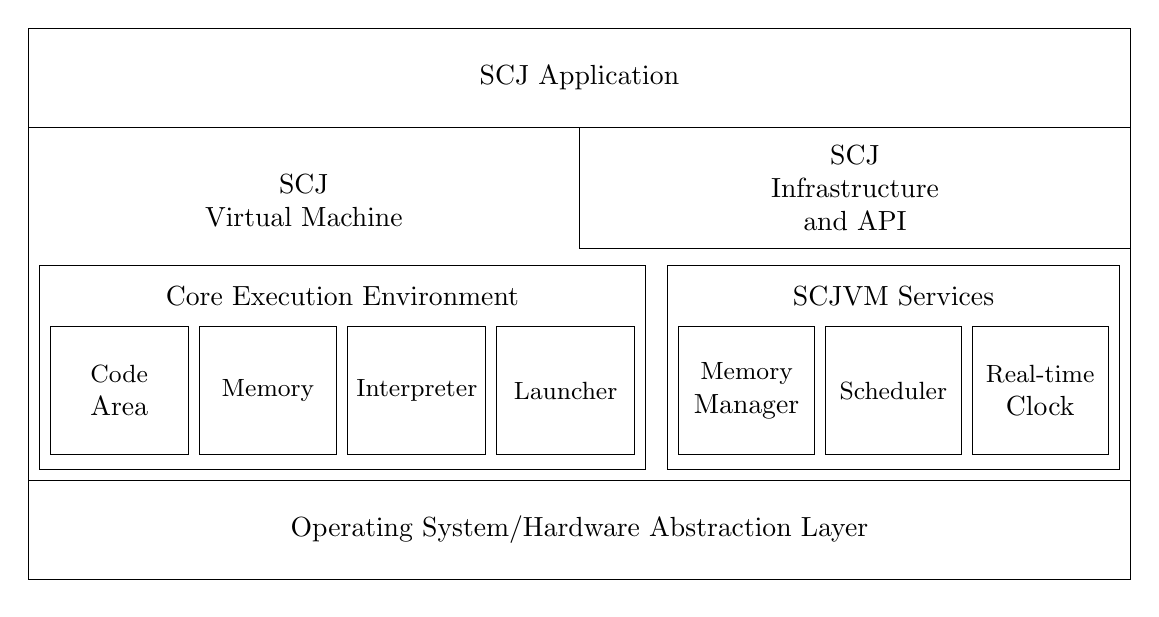
\begin{tikzpicture}

    \coordinate (width)  at (14cm,0cm);
    \coordinate (height) at (0cm,7cm);

    \path (0,0) -- (height)
    coordinate[pos=0.18] (OS boundary)
    coordinate[pos=0.20] (VM part bottom)
    coordinate[pos=0.57] (VM part top)
    coordinate[pos=0.60] (API boundary)
    coordinate[pos=0.82] (App boundary);
    
    \path (VM part bottom) -- (VM part top)
    coordinate[pos=0.7] (VM Service top)
    coordinate[pos=0.7] (CEE part top);

    \path (VM part bottom) -- (VM part top)
    coordinate[pos=0.85] (CEE ypos)
    coordinate[pos=0.85] (VM Services ypos);

    \path (0,0) -- (width)
    coordinate[pos=0.01] (CEE left)
    coordinate[pos=0.56] (CEE right)
    coordinate[pos=0.58] (VM Services left)
    coordinate[pos=0.99] (VM Services right)
    coordinate[pos=0.01] (CEE part sep)
    coordinate[pos=0.01] (VM Service sep);

    \path (CEE left) -- (CEE right)
    coordinate[pos=0.5] (CEE xpos);

    \path (VM Services left) -- (VM Services right)
    coordinate[pos=0.5] (VM Services xpos);

    \path (0,0) to node[pos=0.5] (mid) {} (width);
    \path (0,0) to node[pos=0.25] (quart) {} (width);

    \draw (0,0) rectangle (width |- height);

    \draw (OS boundary) -- ++(width);
    \path (0,0) rectangle node[pos=0.5] (OS) {} (width |- OS boundary);
    \draw (mid |- API boundary) rectangle node[pos=0.5] (API) {} (width |- App boundary);
    \draw (App boundary) -- ++(width);
    \path (App boundary) rectangle node[pos=0.5] (App) {} (width |- height);

    \path (quart |- API boundary) rectangle node[pos=0.4] (SCJVM) {} (quart |- App boundary);
    \draw (VM Services left |- VM part bottom) rectangle (VM Services right |- VM part top);
    \draw (CEE left |- VM part bottom) rectangle (CEE right |- VM part top);
    \coordinate (CEE) at (CEE xpos |- CEE ypos);
    \coordinate (VM Services) at (VM Services xpos |- VM Services ypos);

    \node[align=center] at (App)   {SCJ Application};
    \node[align=center] at (API)   {SCJ\\Infrastructure\\and API};
    \node[align=center] at (SCJVM) {SCJ\\Virtual Machine};
    \node[align=center] at (CEE)   {Core Execution Environment};
    \node[align=center] at (VM Services)  {SCJVM Services};
    \node[align=center] at (OS)    {Operating System/Hardware Abstraction Layer};
    
    \foreach \x in {1,...,4}
    \pgfmathsetmacro{\a}{0.25*(\x - 1)}
    \pgfmathsetmacro{\b}{0.25*\x}
    \path ($(CEE left) + (VM part bottom)!0.07!(VM part top)$) -- 
    node[pos=\a] (CEE part \x start) {}
    node[pos=\b] (CEE part \x end) {}
    ($(CEE right) + (VM part bottom)!0.07!(VM part top) - (CEE part sep)$);

    \foreach \x in {1,...,4} 
    \draw ($(CEE part \x start) + (CEE part sep)$)
    rectangle node[pos=0.5] (CEE part \x) {}
    (CEE part \x end |- CEE part top);

    \node[align=center] at (CEE part 1) {\small Code\\Area};
    \node[align=center] at (CEE part 2) {\small Memory};
    \node[align=center] at (CEE part 3) {\small Interpreter};
    \node[align=center] at (CEE part 4) {\small Launcher};

    \foreach \x in {1,...,3}
    \pgfmathsetmacro{\a}{0.333*(\x - 1)}
    \pgfmathsetmacro{\b}{0.333*\x}
    \path ($(VM Services left) + (VM part bottom)!0.07!(VM part top)$) -- 
    node[pos=\a] (VM Service \x start) {}
    node[pos=\b] (VM Service \x end) {}
    ($(VM Services right) + (VM part bottom)!0.07!(VM part top) - (VM Service sep)$);

    \foreach \x in {1,...,3} 
    \draw ($(VM Service \x start) + (VM Service sep)$)
    rectangle node[pos=0.5] (VM Service \x) {}
    (VM Service \x end |- VM Service top);

    \node[align=center] at (VM Service 1) {\small Memory\\Manager};
    \node[align=center] at (VM Service 2) {\small Scheduler};
    \node[align=center] at (VM Service 3) {\small Real-time\\Clock};
  \end{tikzpicture}
  \caption{A diagram showing the structure of an SCJVM and its
    relation to the SCJ infrastructure and the operating
    system/hardware abstraction layer}
  \label{scjvm-fig}
\end{figure}

The creation of a specification for the SCJVM services will be
described in Section~\ref{scjvm-services-progress-section}, followed
by a description of work on a specification of the core execution
environment in Section~\ref{cee-progress-section}.
Finally, other activities not directly related to the main research
are discussed in Section~\ref{other-activities-section}

\section{Safety-Critical Java Virtual Machine Services}
\label{scjvm-services-progress-section}

We have elicited the requirements related to the SCJVM services first
as the core execution environment needs to make use of them.
We identified the necessary services by considering the services
offered by the SCJ API given in the SCJ standard~\cite{locke2013} and
identifying the low-level virtual machine services that are necessary
to support them.
This work has been carried out in close consultation with the
standardisation group.
The services have been divided into three areas, as can be seen in
Figure~\ref{scjvm-fig}: the memory manager, the scheduler and the
real-time clock.
This division of services is usual for real-time systems~\cite{li2003}
and matches the chapters of the SCJ standard.
We do not handle the device access services of SCJ as the device
interaction model has not yet been finalised.
Our identification of the required SCJVM services and their behaviour
was checked with a member of the SCJ committee.

We have also collaborated in some work carrying out an in-depth study
of the icecap HVM, which is, to the best of our knowledge, the only
publicly available up-to-date SCJVM.
This has helped in understanding the architecture of an SCJVM and
provided inspiration for our definition of the SCJVM service
requirements.
The study of the icecap HVM included a partial verification effort
using \Circus{} and focusing on the scheduler.
Results from this work have been submitted to the 12th International
Conference on integrated Formal Methods (iFM
2016)~\cite{freitas2016submitted}.

We have created a formal model of the SCJVM services using the
\Circus{} specification language.
The formal model was created by first specifying the services using Z
and then wrapping them in \Circus{} processes to specify how the
services are accessed and the interactions between them.
One \Circus{} process is used for each of the three areas of SCJVM
services.

The formal model of the memory manager has been partially subjected to
proof using Z/Eves.
The proofs performed take the form of domain check proofs and
consistency proofs, and the first two sections of the memory manager,
covering memory blocks and backing stores, have been covered already.
A few proofs concerning the global memory manager section have also
been done.
Additionally, many theorems about objects in the Z/Eves mathematical
toolkit have been proved in the course of this work.

Overall the SCJVM services model is quite large.
A summary of the number of declarations, theorems and proofs is given
in Table~\ref{scjvm-services-decls-table}, which was generated using
the declaration counting facilities of CZT's \LaTeX{} style.
Note that the number of unboxed items may not be accurate as
declarations on separate lines are counted separately in unboxed
environments and \Circus{} action environments are not counted,
although plain \Circus{} environments are.
The other counts are believed to be correct.
The number of proofs is higher than the number of theorems due to the
fact that domain check proof obligations are generated by Z schemas
without a corresponding theorem.
There are 13 memory manager services, 21 scheduler services and 4
real-time clock services.

\setcounter{cntZtotunboxed}{196}
\setcounter{cntZtotaxdef}{13}
\setcounter{cntZtotgendef}{0}
\setcounter{cntZtotschema}{146}
\setcounter{cntZtotgenschema}{0}
\setcounter{cntZtottheorem}{132}
\setcounter{cntZtotproof}{157}
\setcounter{cntZtotdecl}{644}
\begin{table}[ht]
        \begin{center}
                \begin{tabular}{|l|r|}
                		\ZDeclTblInfoGlobal
                \end{tabular}
        \end{center}
        \caption{Summary of declarations in the SCJVM services model.}
        \label{scjvm-services-decls-table}
\end{table}

The specification and formal model of the SCJVM services can be found
in Chapter~3 of the technical report in Appendix~\ref{techreport} of
this report.
The Z/Eves theorems and proofs can also be found in the appendix of
that report.
The SCJVM services were presented at the 13th International Workshop
on Java Technologies for Real-time and Embedded Systems (JTRES
2015)~\cite{baxter2015a}.

\section{The Core Execution Environment}
\label{cee-progress-section}

Having specified the SCJVM services, we then created a specification
of the core execution environment as a starting point for the
compilation strategy. 
We started by identifying a suitable subset of Java bytecode to work
with.
A subset of Java bytecode is necessary to permit effective reasoning
since Java bytecode and the JVM are very large and complex.
Our subset is large enough to express a wide variety of SCJ programs
and to illustrate how it may be extended with further features.

To inform our choice of bytecode subset, we first compiled a simple
SCJ ``hello world'' program using a standard Java compiler and the
icecap SCJ API implementation~\cite{korsholm2014} and examined the
resultant bytecode.
From the bytecode generated by that example we selected a subset of
Java bytecode, removing instructions that were similar to other
instructions in the subset.
This ensures that we do not unnecessarily complicate the model with
trivial or redundant instructions and better allow ourselves to
concentrate on the instructions that are most of interest in creating
the compilation strategy.
For example, basic arithmetic instructions were left out but method
invocation instructions were included in the subset.

Having selected a bytecode subset, we obtained the semantics of the
instructions by looking at the JVM specification~\cite{lindholm2014}.
Features of SCJ such as disallowing dynamic class loading allow for
simplifications to the semantics of some instructions, such as
simplifying method lookup with precomputed method tables.
We then specified the semantics of each instruction using a Z schema,
with a state based on the JVM specification's descriptions of Java
class files and stack frames.

The Z model of the bytecode subset was then extended to a model of the
interpreter using \Circus{}. 
It was realised that, in order to properly specify the semantics of
some instructions for creation of objects and invocation of some
special methods and ensure that the semantics of the core execution
environment as a whole is specified, it is necessary to model the SCJ
startup process and mission model.
We did this as a separate \Circus{} process called the launcher, which
is responsible for coordinating the execution.
The core execution environment is split into four areas in total, as
seen in Figure~\ref{scjvm-fig}, each represented by a \Circus{}
process:~the code area, the memory, the interpreter and the launcher.
The memory must additionally handle communication with the SCJVM
memory management services and maintain an awareness of which memory
areas are in use to properly coordinate entering and exiting of memory
areas.
The launcher must also communicate with the scheduler as part of
starting missions and coordinating the execution of bytecode
instructions.
So the core execution environment makes use of the SCJVM services
already defined and the \Circus{} model for the core execution
environment must make use of the channels from the SCJVM services
model.

The number of declarations in the core execution environment model is
shown in Table~\ref{cee-decls-table}, counted by the CZT \LaTeX{}
package much as in Table~\ref{scjvm-services-decls-table}.
The core execution environment is a smaller model than the SCJVM
services model, with fewer Z schemas and more reliance on \Circus{}
actions.
The core execution environment has more axiomatic definition
paragraphs than the SCJVM services model as these are used to
introduce special method identifiers and auxiliary functions on given
types representing SCJVM words.
The core execution environment model has not yet been the subject of
proof, though it has been syntax and typechecked using CZT.

\setcounter{cntZtotunboxed}{157}
\setcounter{cntZtotaxdef}{68}
\setcounter{cntZtotgendef}{0}
\setcounter{cntZtotschema}{47}
\setcounter{cntZtotgenschema}{0}
\setcounter{cntZtottheorem}{0}
\setcounter{cntZtotproof}{0}
\setcounter{cntZtotdecl}{272}
\begin{table}[ht]
        \begin{center}
                \begin{tabular}{|l|r|}
                		\ZDeclTblInfoGlobal
                \end{tabular}
        \end{center}
        \caption{Summary of declarations in the core execution
          environment model.}
        \label{cee-decls-table}
\end{table}

The core execution environment model and an explanation of the
bytecode subset chosen can be found in Chapter~4 of the technical
report in Appendix~\ref{techreport} of this report.

\section{Other Activities}
\label{other-activities-section}

In addition to research I have been involved in demonstrating for
several modules, namely:
\begin{itemize}
\item Implementation of Programming Languages (IMPL, Autumn term
  2015--2016)
\item Mathematical Foundations of Computer Science (MFCS, Autumn term
  2015--2016)
\item Programming: Correctness by Construction (PCOC, Autumn and
  Spring terms 2015--2016)
\end{itemize}

I was also involved on the programme committee of the 8th York
Doctoral Symposium on Computer Science (YDS 2015).

I continue to explore a wide range of interests and I hope to be able
to participate in more activities around the department in the future.


\chapter{Research Plan}
\label{research-plan-chapter}

In this chapter we describe the plan for the rest of the research,
explaining each of the steps to be taken and giving and estimate of
the amount of time each will take.

Having already constructed formal models of the SCJVM services and
core execution environment, the bulk of the remaining work centres
around the construction and proof of soundness of the compilation
strategy.
A summary of the tasks involved in this, with an estimate of the time
needed and dates during which the work will be carried out, is given
in Table~\ref{research-plan-table}

\begin{table}[ht]
  \centering
  \begin{tabular}{llll}
    \hline
    Task & Time Needed & Start Date & End Date  \\
    \hline
    Define C subset semantics & 2 months & 2016-02-01 & 2016-03-31 \\
    Develop compilation strategy & 4 months & 2016-04-01 & 2016-07-31 \\
    Hand proofs of compilation rules & 6 months & 2016-07-01 & 2016-12-31 \\
    Mechanise proofs of compilation rules & 3 months & 2016-12-01 & 2017-02-28 \\
    Implementation and example development & 2 months & 2017-03-01 & 2017-04-30 \\
    Writing up results & 5 months & 2017-05-01 & 2017-09-30 \\
    \hline
  \end{tabular}
  \caption{A table showing the proposed plan for the remainder of the research}
  \label{research-plan-table}
\end{table}

\section{C Subset Semantics}

The first task is to define the target language for the compilation
strategy.
As mentioned in Section~\ref{objectives-section}, the focus is on C,
since that is the target language used by several existing SCJVMs.
However, since C is being used as a target language and not as a
high-level source language, not all features of C will be required.
This means that we must first determine a subset of C that will be
sufficiently powerful to support the compilation but sufficiently
small to permit reasoning.

The C subset will be determined by consideration of the parts of C
used by existing SCJVMs such as the icecap HVM.
We will also do some preliminary thinking about the compilation
strategy at this stage to identify the parts of C required for it.

Once the C subset is determined, its semantics must be defined.
In order to apply the algebraic approach, the semantics must be
described in the same semantic space as the source language and SCJVM,
model so that there will be a refinement relation between them.
This means an existing C semantics cannot necessarily be used
as-is:~we need a \Circus{} semantics.

Nevertheless, consideration of existing C semantics can be of use in
defining the semantics of our subset.
This is particularly true in light of the fact that the generated C
code, generated by applying the compilation strategy will then need to
be compiled correctly.
So, it is wise to ensure that our semantics is a valid account of the
accepted semantics of the subset of C of interest.
We will validate our C semantics by comparing it to existing models of
the semantics of C and carefully checking it against the C standard.
The soundness of the semantics will be ensured by the same proof
techniques as for the SCJVM model.
Overall, due to the small size of our subset and the fact that some
existing models of C semantics can be referenced, we do not expect the
process of defining the subset and its semantics to take very long and
so we have allotted two months for it.

\section{Development of Compilation Strategy}

The next task is the construction of the compilation strategy to go
from the source language to the target language.
The approach taken in earlier works using the algebraic
approach~\cite{sampaio1993,duran2005} is to divide the compilation
into stages with compilation rules for each stage.
This is a sensible approach to adopt in developing the compilation
strategy, so we will proceed by identifying the main transformations
that must be performed and then breaking them down into specific rules
to transform each program element.
As this is a significant part of our research, we have allowed four
months for it.

Additionally, while constructing the compilation strategy, we will
also construct some example SCJ programs that can be used as case
studies for the compilation strategy.
This will support us in ensuring that the compilation strategy is
designed to work for actual programs and it also means the
compilation strategy can be easily compared to existing SCJVMs.

\section{Proof of Compilation Rules}

While the top-down approach described above enables construction of
the compilation strategy, proof of its correctness must follow a 
bottom-up approach starting from basic axioms and using
those to prove the compilation rules.
With that in mind, the next stage after drawing up the compilation
strategy is to prove it sound.
Because machine-checked proofs can take a long time to write and
hand-written proofs can be better for reading and understanding,
we will initially construct proofs by hand before translating them
into an automated theorem prover.
We have allowed six months for the hand-written proofs as they may be
difficult to construct and form an important part of the work.

The hand-written proofs then need to be performed in an automated
theorem prover in order to have them machine-checked.
The theorem prover we will use is Isabelle, due to the fact that it is
well developed and there is an implementation of UTP in Isabelle that
can be used to work with \Circus{}.
We have allowed three months for completing this stage of the proof as
Isabelle provides a lot of proof automation and the main outline of
the proofs should already exist from the previous stage.

\section{Implementation and Example Development}

With the main task of developing and proving the compilation strategy
performed, we will implement the compilation strategy.
This should be a relatively simple task since the compilation rules
will take the form of rewrite rules that can be turned into functions.
Isabelle's code generation facilities can be used to check the
functions against the proved compilation laws and convert them to
executable code.
At this stage more work can also be done developing example SCJ
programs whose bytecode can then be passed through the implementation
of the compilation strategy and the output compared to that of other
SCJVMs.
We have allowed two months for this work.

\section{Writing Up Results}

Finally, we have left five months at the end of the project for final
writing up of results.
However, the main writing up effort will be carried out as part of the
other stages of the work.
If there is any extra time available, it would be good to implement
additional bytecode instructions not in the original subset at this
stage, especially if they may be required by the examples we create.

In conclusion, upon successful completion of this work we will have
created a framework that will allow creation of a formally verified
virtual machine for SCJ.
This will offer a certainty of correctness not offered by existing
SCJVMs and so facilitate the use of SCJ.

\begin{sidewaysfigure}
\centering
\begin{minipage}{\textheight}
\centering
\begin{ganttchart}[
  vgrid,
  x unit=0.7cm,
  time slot format = isodate-yearmonth,
  compress calendar
  ]{2016-01}{2017-12}
  \gantttitlecalendar{year, month=shortname} \\
  \ganttbar{Define C subset semantics}{2016-02}{2016-03} \\
  \ganttbar{Develop compilation strategy}{2016-04}{2016-07} \\
  \ganttbar{Hand proofs of compilation rules}{2016-07}{2016-12} \\
  \ganttbar{Mechanise proofs of compilation rules}{2016-12}{2017-02} \\
  \ganttbar{Implementation and example development}{2017-03}{2017-04} \\
  \ganttbar{Writing up results}{2016-03}{2016-03}
  \ganttbar{}{2016-07}{2016-07}
  \ganttbar{}{2017-05}{2017-09} \\
\end{ganttchart}
\end{minipage}
\caption{A Gantt chart showing the schedule for the planned research}
\end{sidewaysfigure}

\printbibliography

\appendix

\chapter{Paper submitted to iFM 2016}
\label{ifmpaper}

\includepdf[pages=-]{../../SCJ-VM/rtss/icecap-scj.pdf}

\chapter{Technical Report}
\label{techreport}

\includepdf[pages=-]{../Qualifying-Dissertation/qualifyingdissertation.pdf}

\end{document}